\documentclass[aps,twocolumn,secnumarabic,amsmath,amssymb]{revtex4}
\usepackage{amsmath}
\usepackage{amssymb}
\usepackage{amsfonts}
\usepackage{color}
\usepackage{graphics}
\usepackage[pdftex]{graphicx}
\usepackage[utf8x]{inputenc}
\usepackage[colorlinks=true]{hyperref}

\newcommand{\ud}{\mathrm{d}}
\newcommand{\ue}{\mathrm{e}}
\newcommand{\ui}{\mathrm{i}}
\newcommand{\res}{\mathrm{Res}}
\newcommand{\Tr}{\mathrm{Tr}}
\newcommand{\dsum}{\displaystyle\sum}
\newcommand{\dprod}{\displaystyle\prod}
\newcommand{\dlim}{\dispqlaystyle\lim}
\newcommand{\dint}{\displaystyle\int}
\newcommand{\fsno}[1]{{\!\not\!{#1}}}
\newcommand{\texp}[2]{\ensuremath{{#1}\times10^{#2}}}
\newcommand{\dexp}[2]{\ensuremath{{#1}\cdot10^{#2}}}
\newcommand{\eval}[2]{{\left.{#1}\right|_{#2}}}
\newcommand{\paren}[1]{{\left({#1}\right)}}
\newcommand{\lparen}[1]{{\left({#1}\right.}}
\newcommand{\rparen}[1]{{\left.{#1}\right)}}
\newcommand{\abs}[1]{{\left|{#1}\right|}}
\newcommand{\sqr}[1]{{\left[{#1}\right]}}
\newcommand{\crly}[1]{{\left\{{#1}\right\}}}
\newcommand{\angl}[1]{{\left\langle{#1}\right\rangle}}
\newcommand{\tpdiff}[4][{}]{{\paren{\frac{\partial^{#1} {#2}}{\partial {#3}{}^{#1}}}_{#4}}}
\newcommand{\tpsdiff}[4][{}]{{\paren{\frac{\partial^{#1}}{\partial {#3}{}^{#1}}{#2}}_{#4}}}
\newcommand{\pdiff}[3][{}]{{\frac{\partial^{#1} {#2}}{\partial {#3}{}^{#1}}}}
\newcommand{\diff}[3][{}]{{\frac{\ud^{#1} {#2}}{\ud {#3}{}^{#1}}}}
\newcommand{\psdiff}[3][{}]{{\frac{\partial^{#1}}{\partial {#3}{}^{#1}} {#2}}}
\newcommand{\sdiff}[3][{}]{{\frac{\ud^{#1}}{\ud {#3}{}^{#1}} {#2}}}
\newcommand{\tpddiff}[4][{}]{{\left(\dfrac{\partial^{#1} {#2}}{\partial {#3}{}^{#1}}\right)_{#4}}}
\newcommand{\tpsddiff}[4][{}]{{\paren{\dfrac{\partial^{#1}}{\partial {#3}{}^{#1}}{#2}}_{#4}}}
\newcommand{\pddiff}[3][{}]{{\dfrac{\partial^{#1} {#2}}{\partial {#3}{}^{#1}}}}
\newcommand{\ddiff}[3][{}]{{\dfrac{\ud^{#1} {#2}}{\ud {#3}{}^{#1}}}}
\newcommand{\psddiff}[3][{}]{{\frac{\partial^{#1}}{\partial{}^{#1} {#3}} {#2}}}
\newcommand{\sddiff}[3][{}]{{\frac{\ud^{#1}}{\ud {#3}{}^{#1}} {#2}}}
\newcommand{\eff}{ef\! f}

\begin{document}
\title{Motional Quantum Ground-State Cooling Outside the Lamb-Dicke Regime -- Supplemental material}
\author{Yichao Yu}
\author{Nicholas R. Hutzler}
\altaffiliation{Present address: California Institute of Technology, Division of Physics, Mathematics, and Astronomy.  Pasadena, CA, 91125}
\author{Jessie T. Zhang}
\author{Lee R. Liu}
\author{Kang-Kuen Ni}
\email{ni@chemistry.harvard.edu}
\affiliation{Department of Chemistry and Chemical Biology, Harvard University, Cambridge, Massachusetts, 02138, USA}
\affiliation{Department of Physics, Harvard University, Cambridge, Massachusetts, 02138, USA}
\affiliation{Harvard-MIT Center for Ultracold Atoms, Cambridge, Massachusetts, 02138, USA}

\date{\today}

\maketitle

\section{Simulation of 3D Raman sideband cooling}

We use a computer simulation to study the importance of different effects
and guide the optimization of Raman sideband cooling.
The simulation uses the quantum jump (or Monte-Carlo wavefunction) method~\cite{Chretien2014}
to accurately calculate the evolution within each laser pulse where different energy eigenstates
are assumed to decohere immediately upon spontaneous emission and on pulse boundaries.
Such approximations are valid and greatly simplify the computation
at the cost of limiting the applicability of the simulation to processes that require stronger
coherence, such as Ramsey spectroscopy or rapid push-out of the atoms from the trap
(faster than a trap oscillation period).

A number of other simplifying approximations, listed below, are also used in the simulation.
These either have a demonstrably negligible effect on the experiment,
or result in a significant reduction of complexity for an effect
that can be optimized more easily in the experiment.

\begin{enumerate}
\item \emph{All Raman pulses resonantly drive only one sideband/carrier order.}  We tweak the pulse shape, power and length as discussed in the text, for example by using Blackman pulses, to reduce coupling to other orders. We do see deviation from this approximation in the experiment, though mostly in the long detection pulses, and it is less of a concern for the short cooling pulses.
\item \emph{No heating from other sources.}\\
  We measured the heating rate and found that it results mainly from off-resonant scattering
  of photons, which is included in the simulation.  In particular, we can ignore heating from the switching trap.
\item \emph{Same trapping frequency for all states.}\\
  This effect is negligible for Na in the ground state due to the small fine structure splitting in the excited state.
  It is straightforward to include this effect if the calculation needs to be repeated
  on a system where this is not the case (e.g. directly laser cooled molecules).
\end{enumerate}

Some effects that are important to include are all three dimensions (3D motional states,
accurate 3D wavevector, and different emission pattern for different photon polarizations),
off-resonant scattering from all laser beams, and optical pumping polarization imperfection.
The optical pumping polarization and off-resonant scattering are especially important
for accurate simulation since they are the main limitation on cooling performance.

In general, each pulse has a coherent part from the Raman drive
(which is absent for the optical pumping pulses)
and an incoherent part from scattering (optical pumping or off-resonant).
This nicely fits the general approach of the quantum jump method.
Due to the large number of states that we need to take into account
($30-150$ motional per axis and $8$ hyperfine, giving a total of $10^6$),
generic wavefunction propagation is very inefficient.
Therefore, we further simplify by reducing the number of states tracked during
the coherent propagation and applying quantum jumps using a set of reduced jump operators that
describe the total jump probability from a certain state (summed over all final states).
The coherent propagation is then accurately solved in order to avoid having to use a time step
much shorter than the inverse of scattering rate (up to hundreds of kHz)\footnote{\href{https://goo.gl/EZ13wt}{note about modification to the quantum jump method (https://goo.gl/EZ13wt)}}.

In order to simulate a pulse, we first start with the coherent propagation that includes the
modification from the jump operators as in the quantum jump method.
When a jump happens, we pick a final internal state to jump to based on the relative rates
of different scattering sources and their branching ratios.
This process determines the polarization and emission pattern of the emitted photon,
from which we randomly sample a particular wave vector.
The photon recoil being defined, we can then assign a final motional state to the atom.
This process is then repeated as long as the pulse is on,
before we start to simulate the next pulse.

We apply ``virtual'' measurements on the results of each simulated cooling sequence
which we then average to obtain the expected value of experimental quantities.
Due to the decoherence approximation, the measurement has to commute with the Hamiltonian.
Particularly useful measurements used in our simulation are hyperfine state distribution,
average motional energy, loss rate (where an atom is assumed to be lost if its motional energy
goes above a certain threshold at any time) probability of being in certain states
(e.g. ground state).

\begin{figure}[t]
  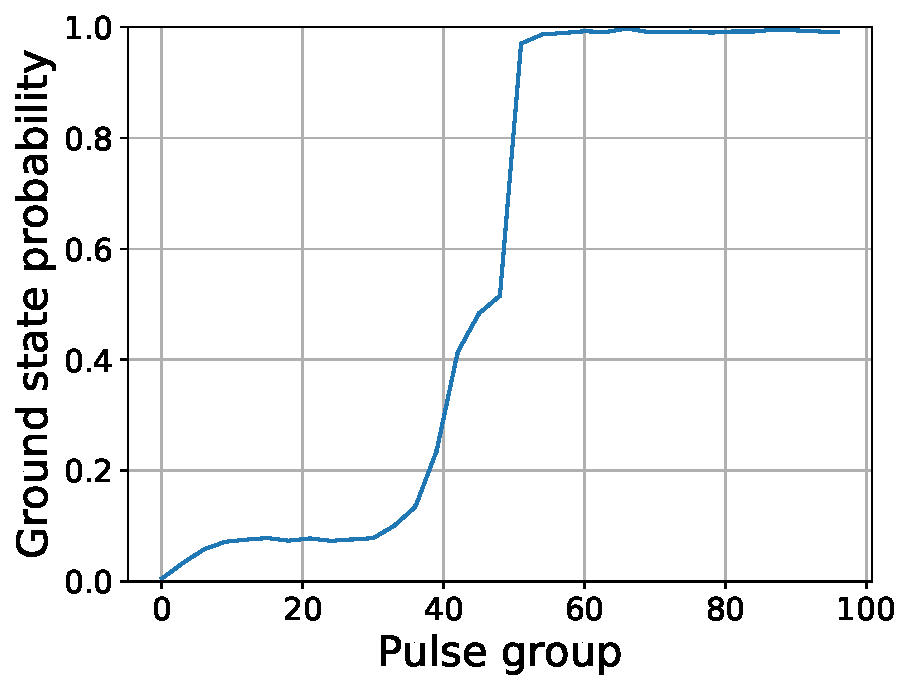
\includegraphics[width=8.5cm]{imgs/simcool_no_scatter.pdf}
  \caption{Simulated 3D ground state population as a function of cooling cycles without
    technical imperfections. The ground state probability reaches $>99\%$. \label{f-no-scatter}}
\end{figure}
\begin{figure}[t]
  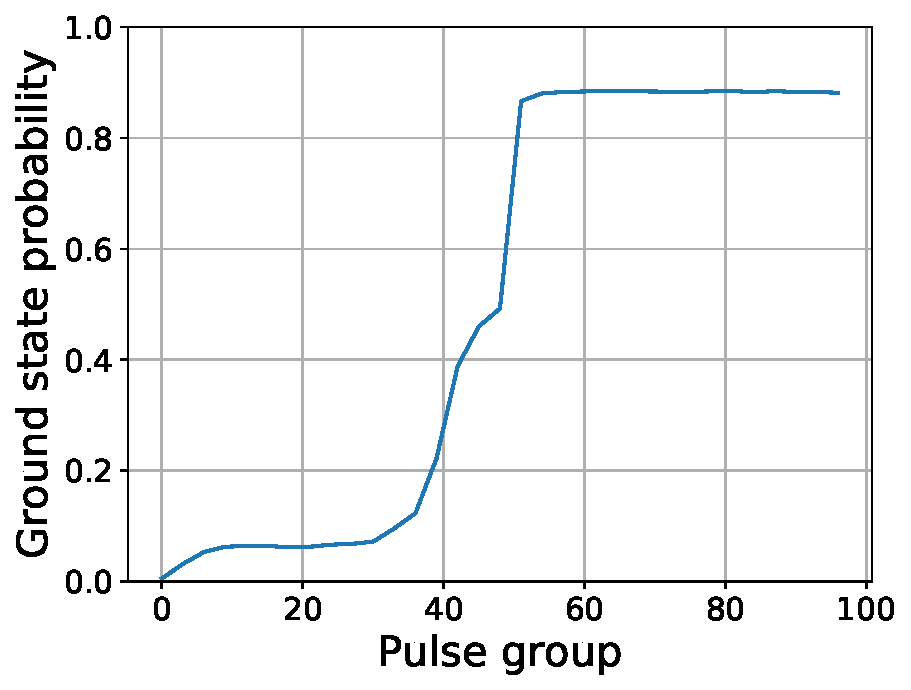
\includegraphics[width=8.5cm]{imgs/simcool_real.pdf}
  \caption{Simulated 3D ground state population as a function of cooling cycles including effect of
    off-resonant scattering from all beams and OP misalignment.
    For this particular sequence, the ground state probability saturates to $\approx88\%$.
    \label{f-real}}
\end{figure}

If off-resonant scattering and optical pumping polarization misalignment are ignored,
the simulation shows that there is not a cooling limit
despite the large Lamb-Dicke parameter and high initial temperature (Fig \ref{f-no-scatter}).
However, when these effects are taken into account, the ground state probability can saturate at
a lower value (Fig \ref{f-real}) and require much more careful tweaking.
The change of slop in these plots corresponds to changing the sideband orders used for cooling.

The simulation is written in Julia\cite{Bezanson2017}.
All code is available under the GPLv3 license at
\footnote{\href{https://goo.gl/WLJwJp}{Library code (https://goo.gl/WLJwJp)}} and
\footnote{\href{https://goo.gl/XXVreq}{Top level code (https://goo.gl/XXVreq)}}

% mention effects that are included first?

\bibliography{paper}
\end{document}
